\chapter{Teoría del MLR}

\section{Introducción}
Teniendo en cuenta que el trabajo realizado contempló el diseño, optimización y control de un MLR, fue necesario realizar un estudio exhaustivo de la teoría detrás de su funcionamiento con el fin de adquirir un entendimiento que sirviera como soporte para los objetivos planteados. Este estudio se llevó a cabo a partir de consultas con profesionales en el área, libros de texto y artículos de divulgación. Con el fin de concentrar el contenido principal del libro en los resultados del trabajo, la teoría se ha pasado a este apéndice y se desarrolla a continuación.

\section{Modelo matemático del MLR}
El primario del MLR diseñado consiste de un devanado trifásico distribuido. Cada uno de los devanados por fase es una bobina que puede modelarse como una resistencia $R_s$ en serie con una inductancia $L_s$, como se muestra en la Fig. \ref{fig:primarycircuit}. De esta forma, el voltaje total es igual a la caída de voltaje en la resistencia más el voltaje inducido en la bobina \cite{fitzgerald2003}.
\begin{figure}[t]
\centering
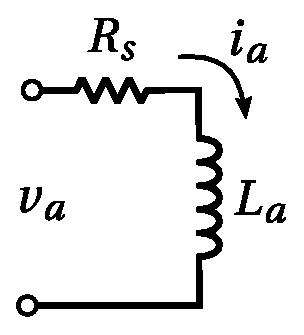
\includegraphics[scale=0.5]{../img/Teoria_del_MLR/primarycircuit.eps}
\caption{Circuito equivalente de la bobina del primario para una fase}
\label{fig:primarycircuit}
\end{figure}
Esta relación puede escribirse como
\begin{align*}
v_a &= R_s i_a + e_a\\
&= R_s i_a + \frac{d\lambda_a(x)}{dt}
\end{align*}
donde $e_a$ es el voltaje inducido y $\lambda_a$ es el flujo de enlace. Debido a la propiedad anisotrópica del secundario, la inductancia $L_a$, y consecuentemente el flujo de enlace $\lambda_a$ son funciones de la posición $x$, lo que dificulta el modelamiento matemático y el control del MLR si se intenta trabajar de esta forma.

Con el fin de simplificar el modelo dependiente de la posición mostrado anteriormente, puede utilizarse la \textbf{transformación de Park} (también conocida como la transformación \textbf{dq0}), propuesta inicialmente por R. H. Park en \cite{park1929}. Esta es una transformación lineal en la que cantidades desde el punto de vista del primario y las tres fases $a$, $b$ y $c$, se pasan al marco de referencia del secundario que se mueve a velocidad síncrona. Esta transformación es dependiente de la posición, pero produce componentes en el nuevo marco de referencia, que son independientes de la posición. Este nuevo marco de referencia contiene dos ejes, uno alineado con el eje magnético de la fase $a$, y otro a 90° del eje magnético de la fase $a$. Estos ejes se conocen como el eje \textbf{directo} y en \textbf{cuadratura}, respectivamente. Existe un eje adicional, conocido como el eje de secuencia cero, que en sistemas balanceados es cero.

La matriz que permite obtener la transformación del eje $abc$ al eje $dq$ es la siguiente, donde $S$ puede ser cualquier variable eléctrica o magnética, como un voltaje, corriente o flujo de enlace:
\begin{equation}
\begin{bmatrix}
S_d\\ 
S_q\\ 
S_0
\end{bmatrix}
=\frac{2}{3}
\begin{bmatrix}
\cos(\theta_{me}) & \cos(\theta_{me}-120^\circ) & \cos(\theta_{me}+120^\circ)\\
-\sin(\theta_{me}) & -\sin(\theta_{me}-120^\circ) & -\sin(\theta_{me}+120^\circ)\\
\frac{1}{2} & \frac{1}{2} & \frac{1}{2}
\end{bmatrix}
\begin{bmatrix}
S_a\\ 
S_b\\ 
S_c
\end{bmatrix}
\end{equation}

Al aplicar esta transformación, las corrientes del primario pueden descomponerse en sus componentes en el eje directo y en cuadratura, $i_d$ e $i_q$, el flujo de enlace del primario en las componentes $\lambda_d$ y $\lambda_q$, y el voltaje en las componentes $v_d$ y $v_q$. La aplicación de la transformación dq0 permite obtener las dos siguientes ecuaciones para los voltajes en los ejes directo y en cuadratura:
\begin{align*}
v_d &= R_s i_d + \frac{d\lambda_d}{dt} - v_{me}\lambda_q\\
v_q &= R_s i_q + \frac{d\lambda_q}{dt} + v_{me}\lambda_d
\end{align*}
donde $v_{me}$ es la frecuencia de línea y $v_{me} = \frac{d\theta_{me}}{dt}$, y $\theta_{me}$ es el número de grados eléctricos entre el eje magnético de la fase a y el eje d, que como función de la posición en el MLR puede escribirse como
\begin{equation*}
\theta_{me} = \frac{\pi}{\tau}x
\end{equation*}
Los flujos de enlace en los ejes directo y en cuadratura pueden escribirse como
\begin{align*}
\lambda_d &= L_d i_d\\
\lambda_q &= L_q i_q
\end{align*}

En estado estacionario, las derivadas del flujo de enlace en los ejes d y q se hacen cero, por lo que las ecuaciones de los voltajes en los ejes d y q se pueden escribir en estado estacionario como
\begin{align}
V_d &= R_s I_d - v_{me}L_q I_q\\
V_q &= R_s I_q + v_{me}L_d I_d
\end{align}

\section{El coeficiente de saliencia}
Al obtener las relaciones de torque y potencia en los motores síncronos rotatorios, la suposición inicial es que el rotor es cilíndrico, lo que implica que su reluctancia es constante alrededor de su perímetro \cite{chapman2003}. Esto aplica igualmente en los motores síncronos lineales. En configuraciones más complejas, como secundarios con polos salientes, esta suposición deja de ser aplicable, por lo que es necesario encontrar nuevamente relaciones para el torque la potencia en el caso en el que el rotor no puede considerarse cilíndrico y la reluctancia es variable a lo largo del secundario. Una solución consiste en separar las componentes de los campos en una componente alineada con el eje del secundario con la máxima reluctancia, y otra componente perpendicular a este eje, por medio de la transformación dq0 \cite{gieras2000}.

Al realizar esta separación, la potencia electromagnética puede escribirse como
\begin{equation}
P_e = m_1\left( \frac{V_1 E_f}{X_{sd}}\sin\delta
+ \frac{V_1^2}{2}\left( \frac{1}{X_{sq}} - \frac{1}{X_{sd}}\right)\sin(2\delta) \right)
\label{potenciaem}
\end{equation}
donde $m_1$ es el número de fases, $V_1$ es el voltaje de fase, $E_f$ es el voltaje inducido, $X_{sd}$ y $X_{sq}$ son las inductancias del eje directo y en cuadratura, respectivamente, y $\delta$ es el ángulo de carga. Como puede verse, la potencia tiene dos componentes, una debida al torque síncrono, y otra debida al torque de reluctancia. En un motor de reluctancia, como el MLR, $E_f = 0$, debido a que no hay una fuente externa de campo magnético, y el empuje inducido es
\begin{equation}
F_{ind} = \frac{P_e}{v}
\end{equation}
donde $v$ es la velocidad del movimiento, que para un motor lineal es
\begin{align*}
v &= 2\tau f \\
&= \frac{\pi}{\tau}\omega
\end{align*}
donde $\tau$ es el paso polar, $f$ es la frecuencia de la fuente de alimentación en Hertz, y $\omega$ la frecuencia angular en radianes por segundo.

De esta forma, el empuje inducido en el MLR puede escribirse como
\begin{align}
F_x &= \frac{\pi}{\tau}\frac{m_1 V_1^2}{2}
\left( \frac{X_{sd}-X_{sq}}{X_{sq}X_{sq}} \right)\sin(2\delta) \notag\\
&= \frac{m_1 V_1^2}{2X_{sd}}\left(\frac{X_{sd}}{X_{sq}-1}\right)\sin(2\delta)
\end{align}

Dada la definición de reactancia, en general, como $X = \omega L$, estas ecuaciones muestran que con el fin de incrementar la potencia desarrollada y el empuje, se requiere una alta diferencia $L_d-L_q$ y razón $L_d/L_q$ entre las inductancias del eje directo $L_d$ y en cuadratura $L_q$. De aquí se define el \textbf{coeficiente de saliencia} como la razón entre estas inductancias: $L_d/L_q$. De acuerdo a \cite{boldea2013}, en términos prácticos para un MLR se requiere como mínimo un coeficiente de saliencia $L_d/L_q \geq 3$, aunque es deseable obtener valores tales que $L_d/Lq > 7$.

\section{El secundario axial laminado anisotrópico}

Con el fin de incrementar el coeficiente de saliencia en los MLR, se han propuesto diferentes topologías de secundarios, tales como laminaciones segmentadas \cite{lawrenson1967} y el secundario axial laminado anisotrópico (ALA) \cite{cruickshank1966,hamler1998}, basado en propuestas por Kostko que datan de 1923 \cite{kostko1923}, como el que se muestra en la Fig. \ref{fig:LVRM}. Kim et. al. reportan coeficientes de saliencia mayores a 6 \cite{leekimlee2014} para un secundario ALA.

\begin{figure}[t]
\centering
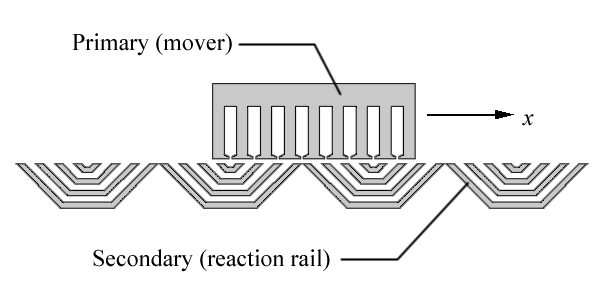
\includegraphics[scale=0.5]{../img/Teoria_del_MLR/LVRM.png}
\caption{MLR con secundario axial laminado anisotrópico}
\label{fig:LVRM}
\end{figure}

En general, para una máquina de polos salientes, las inductancias pueden relacionarse con la inductancia de un secundario uniforme $L_m$, a través de los coeficientes de saliencia para los ejes directo y en cuadratura, al definirse estos como
\begin{align}
k_{dm} &= \frac{L_m}{L_{dm}} \\
k_{qm} &= \frac{L_m}{L_{qm}}
\end{align}
respectivamente, donde $L_{dm}$ y $L_{qm}$ son las inductancias del eje directo y en cuadratura menos la inductancia parásita presente en el motor, es decir,
\begin{align}
L_d &= L_{dm} + L_l \\
L_q &= L_{qm} + L_l
\end{align}

El proceso de diseño adoptado en este trabajo se basó en el método analítico aproximado presentado en \cite{boldea1994}, en el cual se obtiene una relación entre el paso polar $\tau$, la distancia del entrehierro $g$ y los coeficientes de saliencia, tal que
\begin{align}
k_{dm} &= f_1(\tau,g) \\
k_{qm} &= f_2(\tau,g)
\end{align}
Estas funciones son representadas como un conjunto de curvas que fueron utilizadas para seleccionar los valores iniciales para el diseño, como se muestra en las Figs. \ref{fig:kdmvstau} y \ref{fig:kqmvstau}. Teniendo en cuenta que se busca una razón $L_d/L_q$ alta, se concluye de estos resultados que es necesario reducir la distancia del entrehierro, y aumentar el paso polar.

Los coeficientes de saliencia en cada eje pueden también utilizarse para relacionar la densidad de flujo magnético en el entrehierro con un secundario de polos salientes y un secundario uniforme, de forma que
\begin{align}
L_{dm} &= \frac{B_{ed}}{B_e}L_m = k_{dm}L_m \\
L_{qm} &= \frac{B_{eq}}{B_e}L_m = k_{qm}L_m
\end{align}
Existe un efecto más asociado al coeficiente de saliencia $k_{dm}$: debido al incremento del flujo magnético en el eje directo, el secundario se saturará con facilidad, reduciendo el valor efectivo de $k_{dm}$ por un factor de saturación $k_{sd}$ que debe ser estimado durante el diseño \cite{boldea2013}, de forma que el coeficiente de saliencia en el eje directo, incluyendo la saturación, resulta ser
\begin{equation}
k_{dms} = \frac{k_{dm}}{1+k_{sd}}
\end{equation}


\begin{figure}[ht]
\centering
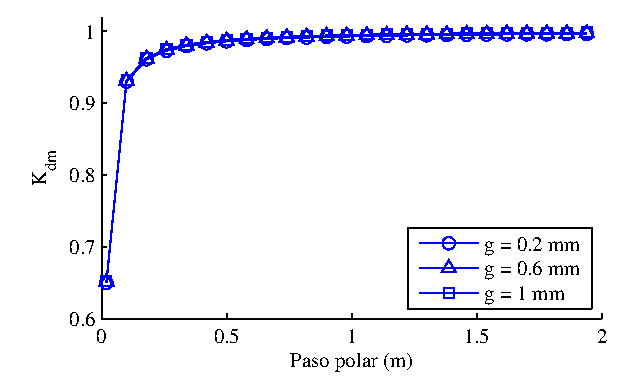
\includegraphics[scale=0.7]{../img/Teoria_del_MLR/kdmvstau.eps}
\caption{Coeficiente de saliencia en el eje directo con respecto al paso polar}
\label{fig:kdmvstau}
\end{figure}

\begin{figure}[ht]
\centering
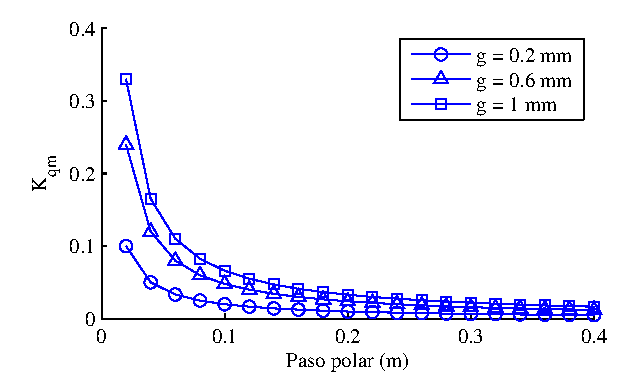
\includegraphics[scale=0.7]{../img/Teoria_del_MLR/kqmvstau.eps}
\caption{Coeficiente de saliencia en el eje en cuadratura con respecto al paso polar}
\label{fig:kqmvstau}
\end{figure}

\section{Maximización del empuje por unidad de flujo}
Una vez se tiene un modelo de parámetros concentrados para el MLR, es posible encontrar una representación fasorial para el mismo, como se sugiere en \cite{boldea2013}. Teniendo en cuenta la ecuación (ecuación diferencial desde el punto de vista del estator), el voltaje del estator $\mathbf{V_s}$ se puede escribir en términos de la resistencia $R_s$, la corriente del estator $\mathbf{I_s}$ y el flujo del estator $\mathbf{\lambda_s}$, en forma fasorial, como
\begin{equation}
\mathbf{V_s} = \mathbf{I_s} R_s + j\omega \mathbf{\lambda_s}
\end{equation}

A partir de esta ecuación se puede obtener un diagrama fasorial, como se muestra en la Fig. \ref{fig:phasordiag}. Esta representación permite obtener otra expresión para la potencia, como alternativa a la presentada en la ecuación \ref{potenciaem}.

\begin{figure}[ht]
\centering
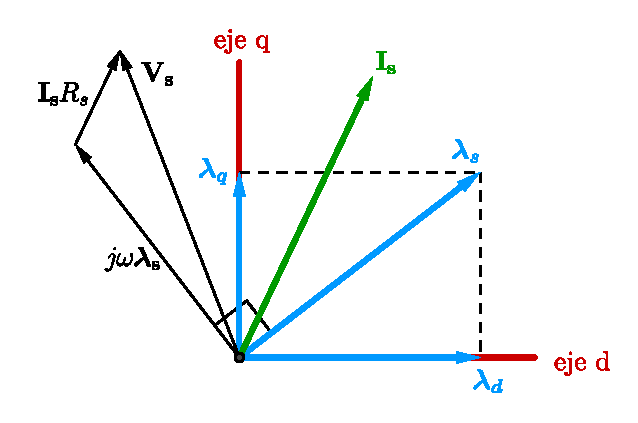
\includegraphics[scale=0.7]{../img/Teoria_del_MLR/phasordiag.eps}
\caption{Diagrama fasorial del MLR.}
\label{fig:phasordiag}
\end{figure}

La potencia de entrada al motor es
\begin{equation}
P = 3\Re\left(\frac{1}{2}\mathbf{V_s}\cdot\mathbf{I_s}^*\right)
\end{equation}
Si la resistencia del estator es despreciable, entonces puede verse del diagrama fasorial que
\begin{equation}
\mathbf{V_s} = j\omega\mathbf{\lambda_s}
\end{equation}
Por lo tanto,
\begin{align}
P &= \frac{3}{2}\Re(j\omega\mathbf{\lambda_s}\cdot\mathbf{I_s}^*)\notag\\
&= \frac{3\omega}{2}\Re(j\mathbf{\lambda_s}\cdot\mathbf{I_s}^*)
\end{align}

La potencia mecánica está dada por
\begin{align*}
P &= F_x v \\
&= F_x 2\tau f \\
&= \frac{\omega\tau}{\pi}F_x
\end{align*}
de forma que
\begin{equation}
F_x = \frac{\pi}{\tau\omega}P
\end{equation}
Por lo tanto, la fuerza puede escribirse como
\begin{align}
F_x &= \frac{\pi}{\tau\omega}
\left(
\frac{3\omega}{2}\Re(j\mathbf{\lambda_s}\cdot\mathbf{I_s}^*)
\right) \notag\\
&= \frac{3\pi}{2\tau}\Re(j\mathbf{\lambda_s}\cdot\mathbf{I_s}^*)
\label{phasorforce}
\end{align}

Teniendo en cuenta que $\mathbf{\lambda_s}=\lambda_d+j\lambda_q$  y $\mathbf{I_s}=I_d+jI_q$, se tiene
\begin{equation}
\mathbf{\lambda_s}=L_d I_d + j L_q I_q
\end{equation}
Por lo tanto,
\begin{align*}
j\mathbf{\lambda_s}\cdot\mathbf{I_s}^* &=
(jL_d I_d-L_q I_q)(I_d-j I_q)\\
&= jL_d I_d^2 + L_d I_d I_q - L_q I_q I_d + j L_q I_q^2
\end{align*}
de forma que
\begin{align*}
\Re(j\mathbf{\lambda_s}\cdot\mathbf{I_s}^*) &= L_d I_d I_q - L_q I_q I_d\\
&= \lambda_d I_q - \lambda_q I_q\\
&= I_d I_q(L_d - L_q)
\end{align*}

Reemplazando en la ecuación \ref{phasorforce}, puede entonces escribirse la fuerza como
\begin{align}
F_x &= \frac{3\pi}{2\tau}(\lambda_d I_q - \lambda_q I_q)\\
&= \frac{3\pi}{2\tau}(L_d - L_q)I_d I_q
\end{align}

Esta última ecuación es un resultado fundamental para el MLR, ya que relaciona directamente las inductancias en el eje directo y en cuadratura, con el empuje ejercido por el motor, y es de gran utilidad durante el diseño, la optimización y el control del motor.

Ahora, si se busca encontrar el valor máximo del empuje por unidad de flujo en el estator, es necesario encontrar una relación entre la fuerza $F_x$ y el flujo $\lambda_s$. Se tiene
\begin{align*}
|\mathbf{\lambda_s}| = \lambda_s &= \sqrt{(L_d I_d)^2+(L_q I_q)^2}\\
&= I_d\sqrt{L_d^2 + (L_q I_q/I_d)^2}\\
&= I_d\sqrt{L_d^2 + (L_q\alpha)^2}
\end{align*}
donde $\alpha = I_q/I_d$. Entonces,
\begin{equation*}
\lambda_s^2 = I_d^2(L_d^2 + (L_q \alpha)^2)
\end{equation*}
y
\begin{equation*}
\lambda_s^2 \alpha = I_d I_q(L_d^2 + (L_q \alpha)^2)
\end{equation*}
de forma que
\begin{equation*}
I_d I_q = \frac{\lambda_s^2 \alpha}{L_d^2 + (L_q \alpha)^2}
\end{equation*}

Entonces, puede escribirse
\begin{equation}
F_x = \frac{3\pi}{2\tau}(L_d - L_q)\frac{\lambda_s^2 \alpha}{L_d^2 + (L_q \alpha)^2}
\label{forcewrtlambda}
\end{equation}
de donde se observa que $F_x$ es máxima si el valor de
\begin{equation*}
\frac{\alpha}{L_d^2+(L_q\alpha)^2} = \frac{\alpha}{m+n\alpha^2}
\end{equation*}
es máximo, donde $m = L_d^2$ y $n=L_q^2$. Para maximizar este valor, se hace
\begin{align*}
\frac{d}{d\alpha}\left\lbrace \frac{\alpha}{m+n\alpha^2} \right\rbrace &= 
\frac{m+n\alpha^2-\alpha(2n\alpha)}{(m+n\alpha^2)^2}\\
&= \frac{m-n\alpha^2}{(m+n\alpha^2)^2} = 0
\end{align*}

De donde se obtiene que
\begin{equation*}
m-n\alpha^2 = 0
\end{equation*}
y
\begin{equation*}
\alpha = \sqrt{m/n}
\end{equation*}


Por lo tanto, para obtener el máximo empuje por unidad de flujo en el estator, se debe cumplir
\begin{align}
\alpha = \frac{I_q}{I_d} &= \sqrt{m/n}\notag\\
&= \sqrt{\frac{L_d^2}{L_q^2}}\notag\\
&= \frac{L_d}{L_q}
\end{align}
o escrito de otra forma,
\begin{equation}
L_d I_d = L_q I_q
\end{equation}

Sabiendo que esta es la condición para el empuje máximo, se puede proceder a encontrar el valor de dicho máximo. Reemplazando $\alpha = L_d/L_q$ en la ecuación \ref{forcewrtlambda}, se obtiene que el valor de empuje máximo es
\begin{align*}
F_{xmax} &= \frac{3\pi}{2\tau}(L_d-L_q)
\frac{\lambda_s^2 (L_d/L_q)}{L_d^2 + (L_q (L_d/L_q))^2} \\
&= \frac{3\pi}{2\tau}(L_d-L_q)\frac{\lambda_s^2}{L_q L_d + L_q L_d}\\
&= \frac{3\pi}{4\tau}\frac{(L_d-L_q)}{L_d L_q}\lambda_s^2\\
&= \frac{3\pi}{4\tau}\frac{(L_d-L_q)}{L_d L_q}\left[ (L_d I_d)^2+(L_q I_q)^2 \right]\\
&= \frac{3\pi}{4\tau}(L_d-L_q)
\left(
I_d^2\frac{L_d}{L_q}+I_q^2\frac{L_q}{L_d}
\right)
\end{align*}
De la condición para el máximo empuje, se tiene $L_d I_d = L_q I_q$, por lo tanto
\begin{equation*}
I_d \frac{L_d}{L_q} = I_q
\end{equation*}
y
\begin{equation*}
I_q \frac{L_q}{L_d} = I_d
\end{equation*}
entonces
\begin{align*}
F_{xmax} &= \frac{3\pi}{4\tau}(L_d-L_q)(I_d I_q + I_d I_q)\\
&= \frac{3\pi}{2\tau} (L_d-L_q)I_d I_q\\
&= \frac{3\pi}{2\tau}L_m
(k_{dms}-k_{qm})I_d I_q
\end{align*}
de acuerdo a la definición de los coeficientes de saliencia en los ejes directo y en cuadratura. La inductancia $L_m$ corresponde a la inductancia de un devanado distribuido \cite{fitzgerald2003}, que puede escribirse como
\begin{equation}
L_m = \frac{6\mu_0(W_1 k_w)^2\tau L}{\pi^2 p k_c g}
\end{equation}
donde y $\mu_0$ es la permeabilidad magnética del espacio vacío (aproximadamente igual a la del aire), $W_1$ es el número de vueltas por devanado en serie, $k_c$ es el coeficiente de Carter, que es introducido para tener en cuenta el incremento en la distancia efectiva del entrehierro debido a las ranuras del primario \cite{boldea2010} y $L$ es el ancho del estator. Reemplazando esta inductancia en la fórmula del empuje máximo, se obtiene
\begin{equation}
F_{xmax} = \frac{18\mu_0 L(k_{dms}-k_{qm})k_w^2 I_d I_q W_1^2}{\pi p k_c g}
\end{equation}

Bajo esta condición, es posible mostrar igualmente  \cite{boldea2013} que el máximo factor de potencia que se puede obtener durante la operación del motor es
\begin{equation}
\cos\phi_{max} = \frac{L_d-L_q}{L_d+L_q}
\end{equation}

\section{Propiedades del devanado}
El factor de devanado se introduce con el fin de tener en cuenta los cambios en la fuerza magnetomotriz producidos por el uso de devanados distribuidos de paso fraccional, en comparación con devanados concentrados de paso completo. El tema es abordado de acuerdo a su presentación en \cite{boldea2010}, aunque existen otras aproximaciones para tener en cuenta estos efectos \cite{chapman2003}, pero que son conceptualmente equivalentes.

En principio, se define el número de ranuras por polo por fase como
\begin{equation}
q = \frac{N_s}{2p_1 m_1}
\end{equation}
donde $N_s$ es el número de ranuras, $p_1$ es el número de pares de polos y $m_1$ es el número de fases. Se denota, por otro lado, el paso de bobina como $y$. Entonces, el factor de distribución $k_d$, que tiene en cuenta el uso de devanados distribuidos en el primario, se define como
\begin{equation}
k_d = \frac{\sin(\pi/6)}{q\sin(\pi/(6q))}
\end{equation}
Además, el factor de encordado, que tiene en cuenta el uso de paso fraccional en los devanados, se define como
\begin{equation}
k_p = \sin\left( \frac{y\pi}{2\tau} \right)
\end{equation}
Finalmente, el factor de devanado, que incluye los dos efectos anteriores, se define como
\begin{equation}
k_w = k_d k_p
\end{equation}

En el caso de los motores lineales con devanado de doble capa, uno de los métodos de devanado causa que existan ranuras con solo una bobina (en lugar de dos), debido a la longitud limitada del primario \cite{gieras2000}. Esto significa que para el mismo número de polos, un motor lineal tiene más ranuras que un motor rotatorio con el mismo número de polos.

En un devanado distribuido de doble capa, generalmente se especifica la razón entre el paso de bobina $y$ y el paso polar $\tau$. Esta razón puede ser fraccional, como por ejemplo, $y/\tau = 5/6$ \cite{boldea2010}. En un motor lineal, un número de polos igual a $y/\tau$ es seleccionado, dividido en dos, y cada unas de estas secciones resultantes es añadida a los extremos del motor. Estas secciones sólo contienen un lado de una bobina. De esta forma, inicialmente el motor cuenta con un número de ranuras $z_0 = 2pmq$. Al añadir las ranuras en los extremos con un solo lado de una bobina, el número total de ranuras es
\begin{equation}
z = \frac{1}{2p}
\left(
2p + \frac{y}{\tau}
\right)
z_0
\end{equation}

\section{Relaciones electromagnéticas en el MLR}

El procedimiento de diseño utilizado plantea la suposición de un valor inicial para el valor pico de la densidad de flujo magnético pico en el entrehierro, $B_{ep}$. Para proceder con el diseño, es necesario encontrar una relación entre esta cantidad y las componentes en el eje directo $B_{epd}$ y en cuadratura $B_{epq}$ de la densidad de flujo magnético en el entrehierro, como se muestra en la figura.
\begin{wrapfigure}{r}{0.2\textwidth}
\centering
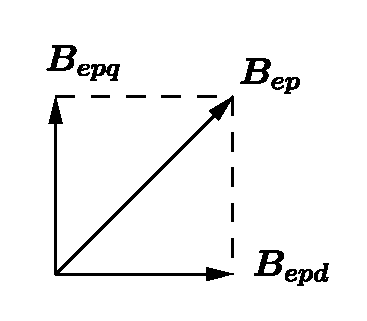
\includegraphics[scale=0.5]{../img/Teoria_del_MLR/B_decomposition.eps}
\end{wrapfigure}
De esta forma, puede escribirse
\begin{equation}
B_{ep}^2 = B_{epd}^2 + B_{epq}^2
\end{equation}
Cada densidad de flujo magnético es proporcional a sus respectivos flujos de enlace $\lambda_{dp}$ y $\lambda_{qp}$, que a su vez son proporcionales a las inductancias en cada eje, $L_{qm}$ y $L_{qms}$, donde en esta última se tiene en cuenta el incremento en la saturación en el eje directo, tal que
\begin{equation}
L_{dms} = \frac{L_{dm}}{1+k_{sd}}
\end{equation}
De esta forma, 
\begin{align*}
B_{epd} &\propto \lambda_{dp} \\
&= L_{dms}I_d\\
&= \frac{L_{dm}}{1+k_{sd}}I_d
\end{align*}
y
\begin{align*}
B_{epq} &\propto \lambda_{qp} \\
&= L_{qm}I_q
\end{align*}
Entonces,
\begin{align*}
B_{ep}^2 &= (L_{dms}I_d)^2 + (L_{qm}I_q)^2\\
&= (L_{dms}I_d)^2\left[1+(I_q/I_d)^2(L_{qm}/L_{dms})^2\right]\\
&= B_{epd}^2\left[1+(I_q/I_d)^2(L_{qm}(1+k_{sd})/L_{dm})^2\right]\\
\end{align*}

Teniendo en cuenta la condición para máximo empuje por unidad de flujo encontrada en la sección anterior, puede entonces expresarse el flujo en el eje directo en términos del flujo en el entrehierro como
\begin{equation}
B_{epd} = \frac{B_{ep}}{\sqrt{1+(I_q/I_d)^2(L_{qm}(1+k_{sd})/L_{dm})^2}}
\end{equation}

La densidad de flujo magnético en el eje directo $B_{epd}$ puede expresarse, por otro lado, mediante el cálculo de la fuerza magnetomotriz $\mathscr{F}_m$ por medio de la ley de Ampere:
\begin{equation*}
\mathscr{F}_m = Ni = \oint_C \mathbf{H}\cdot d\vec{l}
= \frac{1}{\mu}\oint_C\mathbf{B}\cdot d\vec{l}
\end{equation*}
donde $N$ es el número de vueltas, $i$ es la corriente, $\mathbf{H}$ es la intensidad de campo magnético, $C$ es la curva cerrada alrededor de la cual se calcula la integral de línea, $\mu$ es la constante de permeabilidad magnética y $\mathbf{B}$ es la densidad de flujo magnético. Al aplicar esta ley al MLR, la integral puede aplicarse al sistema como se muestra en la Fig. \ref{mmfcalc}.
\begin{figure}[t]
\centering
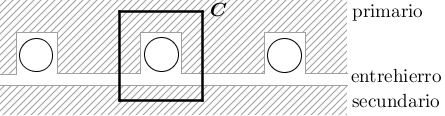
\includegraphics[scale=0.7]{../img/Teoria_del_MLR/mmfcalc}
\caption{Camino de integración en las regiones del MLR}
\label{mmfcalc}
\end{figure}

Asumiendo que la densidad de flujo magnético es uniforme en el entrehierro y que la reluctancia de los materiales ferromagnéticos es despreciable, comparada con la del aire en el entrehierro, se obtiene entonces
\begin{equation*}
\mathscr{F} = \frac{gB}{\mu_0}
\end{equation*}
donde $g$ es la distancia del entrehierro. La densidad de flujo magnético es entonces
\begin{equation}
B = \frac{\mu_0\mathscr{F}}{g}
\end{equation}
Por lo tanto, conociendo la fuerza magnetomotriz, es posible calcular la densidad de flujo magnético. Para un devanado distribuido, la fuerza magnetomotriz está compuesta por una componente fundamental junto con armónicos de orden superior. Una expresión para la fuerza magnetomotriz puede encontrarse a partir del análisis de Fourier, al descomponerla en una serie trigonométrica \cite{boldea2010}. De este análisis, se obtiene que la amplitud de la componente fundamental de la fuerza magnetomotriz es
\begin{equation}
\mathscr{F}_m = \frac{m_1\sqrt{2}W_1 I_a k_w}{\pi p}
\end{equation}
donde $m_1$ es el número de fases, $I_a$ es la corriente de fase y $k_w$ es el factor de devanado (debido a la distribución del devanado y el uso de bobinas de paso fraccional). De esta manera, la densidad de flujo magnético puede escribirse como
\begin{equation}
B_m = \frac{\mu_0 \mathscr{F}_m}{g}
= \frac{\mu_0 3\sqrt{2}W_1 I_a k_w}{\pi g p}
\end{equation}
si el número de fases es 3. Esta densidad de flujo magnético puede descomponerse en componentes en el eje directo y en cuadratura, cada una de las cuales son producidas por corrientes en sus respectivos ejes. En el caso del eje directo, esta componente se puede expresar como
\begin{equation}
B_{epd} = \frac{\mu_0 3\sqrt{2}W_1 I_d k_w}{\pi g p k_c}\cdot
\frac{k_{dm}}{1+k_{sd}}
\end{equation}

\section{Estimación de la masa del motor}
Con el fin de obtener un valor estimado de la masa del motor, es posible iniciar con el cálculo de la cantidad de cobre utilizado en el primario. Durante el proceso de diseño, se obtienen valores para la corriente promedio $I_{av}$ y la densidad de corriente $J_{av}$. Estas cantidades determinan el área transversal de los conductores como $A=I_{av}/J_{av}$. Entonces, el volumen de una sola vuelta es el producto de esta área por la longitud de la misma en una fase. Esta longitud abarca el ancho del motor $L$ y la longitud de las conexiones en los extremos \cite{boldea2013}, definida para cada uno de los dos extremos como
\begin{equation}
L_{ec} = 0.01 + 1.5y
\end{equation}
De esta forma, la longitud total de una vuelta es
\begin{equation}
L_t = 2(L + L_{ec})
\end{equation}
y su volumen es $A L_t$. El número total de vueltas se obtiene al multiplicar el número de vueltas por fase $W_1$ por el número de fases, que usualmente es 3. Finalmente, la masa debida al devanado del primario es el producto entre el volumen y la densidad del cobre $\gamma_c$:
\begin{equation}
M_w = 3W_1\frac{I_{av}}{J_{av}}2(L+0.01+1.5y)\gamma_c
\end{equation}
La masa del núcleo ferromagnético del primario se obtiene al encontrar el área de una sección longitudinal del núcleo y multiplicarla por el ancho del motor para obtener el volumen. Finalmente, se multiplica este volumen por la densidad del material ferromagnético para obtener la masa $M_c$ del mismo. De este modo, la masa del primario (que en el MLR es la parte móvil), es
\begin{equation}
M_p = M_w + M_c
\end{equation}
\bibliographystyle{ieeetr}
\bibliography{../refs}